\begin{center}
    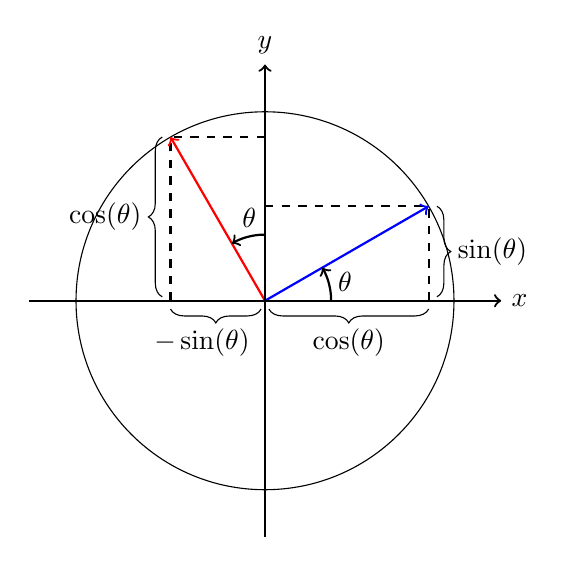
\begin{tikzpicture}[
        vetor/.style = {->, thick},
        braces/.style = {decorate, decoration = {brace, amplitude=5pt, raise=3}}
    ]
        \pgfmathsetmacro{\l}{3}
        \pgfmathsetmacro{\r}{\l*0.8}
        \pgfmathsetmacro{\angulo}{30}

        \draw (0,0) circle (\r);

        \draw[dashed, thick] ({\r*cos(\angulo)},0) -- (\angulo:\r);
        \draw[dashed, thick] (0,{\r*sin(\angulo)}) -- (\angulo:\r);
        
        \draw[dashed, thick] ({-\r*sin(\angulo)},0) -- (\angulo+90:\r);
        \draw[dashed, thick] (0,{\r*cos(\angulo)}) -- (\angulo+90:\r);
        
        \draw[vetor, blue] (0,0) -- (\angulo:\r);
        \draw[vetor, red] (0,0) -- (\angulo+90:\r);

        \draw[vetor] (\r*0.35,0) arc (0:\angulo:\r*0.35) node[right, yshift=-5, xshift=2]{$\theta$};
        \draw[vetor] (0,\r*0.35) arc (90:90+\angulo:\r*0.35) node[above right, yshift=2]{$\theta$};

        \draw [braces] ({\r*cos(\angulo)},0) -- (0.05,0) node[shift={(0,-15pt)}, pos=0.5, black]{$\cos(\theta)$};

        \draw [braces] ({-\r*sin(\angulo)},0.05) -- ({-\r*sin(\angulo)},{\r*cos(\angulo)}) node[left=7pt, pos=0.5]{$\cos(\theta)$};

        \draw [braces, decoration= {mirror}] ({-\r*sin(\angulo)},0) -- (-0.05,0) node[shift={(-5pt,-15pt)}, pos=0.5]{$-\sin(\theta)$};

        \draw [braces, decoration= {mirror}] ({\r*cos(\angulo)},0.05) -- ({\r*cos(\angulo)},{\r*sin(\angulo)}) node[right=7pt, pos=0.5]{$\sin(\theta)$};
        
        \draw[vetor] (-\l,0)--(\l,0) node[right]{$x$};
        \draw[vetor] (0,-\l)--(0,\l) node[above]{$y$};

    \end{tikzpicture}
\end{center}